
% Default to the notebook output style

    


% Inherit from the specified cell style.




    
\documentclass[11pt]{article}

    
    
    \usepackage[T1]{fontenc}
    % Nicer default font (+ math font) than Computer Modern for most use cases
    \usepackage{mathpazo}

    % Basic figure setup, for now with no caption control since it's done
    % automatically by Pandoc (which extracts ![](path) syntax from Markdown).
    \usepackage{graphicx}
    % We will generate all images so they have a width \maxwidth. This means
    % that they will get their normal width if they fit onto the page, but
    % are scaled down if they would overflow the margins.
    \makeatletter
    \def\maxwidth{\ifdim\Gin@nat@width>\linewidth\linewidth
    \else\Gin@nat@width\fi}
    \makeatother
    \let\Oldincludegraphics\includegraphics
    % Set max figure width to be 80% of text width, for now hardcoded.
    \renewcommand{\includegraphics}[1]{\Oldincludegraphics[width=.8\maxwidth]{#1}}
    % Ensure that by default, figures have no caption (until we provide a
    % proper Figure object with a Caption API and a way to capture that
    % in the conversion process - todo).
    \usepackage{caption}
    \DeclareCaptionLabelFormat{nolabel}{}
    \captionsetup{labelformat=nolabel}

    \usepackage{adjustbox} % Used to constrain images to a maximum size 
    \usepackage{xcolor} % Allow colors to be defined
    \usepackage{enumerate} % Needed for markdown enumerations to work
    \usepackage{geometry} % Used to adjust the document margins
    \usepackage{amsmath} % Equations
    \usepackage{amssymb} % Equations
    \usepackage{textcomp} % defines textquotesingle
    % Hack from http://tex.stackexchange.com/a/47451/13684:
    \AtBeginDocument{%
        \def\PYZsq{\textquotesingle}% Upright quotes in Pygmentized code
    }
    \usepackage{upquote} % Upright quotes for verbatim code
    \usepackage{eurosym} % defines \euro
    \usepackage[mathletters]{ucs} % Extended unicode (utf-8) support
    \usepackage[utf8x]{inputenc} % Allow utf-8 characters in the tex document
    \usepackage{fancyvrb} % verbatim replacement that allows latex
    \usepackage{grffile} % extends the file name processing of package graphics 
                         % to support a larger range 
    % The hyperref package gives us a pdf with properly built
    % internal navigation ('pdf bookmarks' for the table of contents,
    % internal cross-reference links, web links for URLs, etc.)
    \usepackage{hyperref}
    \usepackage{longtable} % longtable support required by pandoc >1.10
    \usepackage{booktabs}  % table support for pandoc > 1.12.2
    \usepackage[inline]{enumitem} % IRkernel/repr support (it uses the enumerate* environment)
    \usepackage[normalem]{ulem} % ulem is needed to support strikethroughs (\sout)
                                % normalem makes italics be italics, not underlines
    

    
    
    % Colors for the hyperref package
    \definecolor{urlcolor}{rgb}{0,.145,.698}
    \definecolor{linkcolor}{rgb}{.71,0.21,0.01}
    \definecolor{citecolor}{rgb}{.12,.54,.11}

    % ANSI colors
    \definecolor{ansi-black}{HTML}{3E424D}
    \definecolor{ansi-black-intense}{HTML}{282C36}
    \definecolor{ansi-red}{HTML}{E75C58}
    \definecolor{ansi-red-intense}{HTML}{B22B31}
    \definecolor{ansi-green}{HTML}{00A250}
    \definecolor{ansi-green-intense}{HTML}{007427}
    \definecolor{ansi-yellow}{HTML}{DDB62B}
    \definecolor{ansi-yellow-intense}{HTML}{B27D12}
    \definecolor{ansi-blue}{HTML}{208FFB}
    \definecolor{ansi-blue-intense}{HTML}{0065CA}
    \definecolor{ansi-magenta}{HTML}{D160C4}
    \definecolor{ansi-magenta-intense}{HTML}{A03196}
    \definecolor{ansi-cyan}{HTML}{60C6C8}
    \definecolor{ansi-cyan-intense}{HTML}{258F8F}
    \definecolor{ansi-white}{HTML}{C5C1B4}
    \definecolor{ansi-white-intense}{HTML}{A1A6B2}

    % commands and environments needed by pandoc snippets
    % extracted from the output of `pandoc -s`
    \providecommand{\tightlist}{%
      \setlength{\itemsep}{0pt}\setlength{\parskip}{0pt}}
    \DefineVerbatimEnvironment{Highlighting}{Verbatim}{commandchars=\\\{\}}
    % Add ',fontsize=\small' for more characters per line
    \newenvironment{Shaded}{}{}
    \newcommand{\KeywordTok}[1]{\textcolor[rgb]{0.00,0.44,0.13}{\textbf{{#1}}}}
    \newcommand{\DataTypeTok}[1]{\textcolor[rgb]{0.56,0.13,0.00}{{#1}}}
    \newcommand{\DecValTok}[1]{\textcolor[rgb]{0.25,0.63,0.44}{{#1}}}
    \newcommand{\BaseNTok}[1]{\textcolor[rgb]{0.25,0.63,0.44}{{#1}}}
    \newcommand{\FloatTok}[1]{\textcolor[rgb]{0.25,0.63,0.44}{{#1}}}
    \newcommand{\CharTok}[1]{\textcolor[rgb]{0.25,0.44,0.63}{{#1}}}
    \newcommand{\StringTok}[1]{\textcolor[rgb]{0.25,0.44,0.63}{{#1}}}
    \newcommand{\CommentTok}[1]{\textcolor[rgb]{0.38,0.63,0.69}{\textit{{#1}}}}
    \newcommand{\OtherTok}[1]{\textcolor[rgb]{0.00,0.44,0.13}{{#1}}}
    \newcommand{\AlertTok}[1]{\textcolor[rgb]{1.00,0.00,0.00}{\textbf{{#1}}}}
    \newcommand{\FunctionTok}[1]{\textcolor[rgb]{0.02,0.16,0.49}{{#1}}}
    \newcommand{\RegionMarkerTok}[1]{{#1}}
    \newcommand{\ErrorTok}[1]{\textcolor[rgb]{1.00,0.00,0.00}{\textbf{{#1}}}}
    \newcommand{\NormalTok}[1]{{#1}}
    
    % Additional commands for more recent versions of Pandoc
    \newcommand{\ConstantTok}[1]{\textcolor[rgb]{0.53,0.00,0.00}{{#1}}}
    \newcommand{\SpecialCharTok}[1]{\textcolor[rgb]{0.25,0.44,0.63}{{#1}}}
    \newcommand{\VerbatimStringTok}[1]{\textcolor[rgb]{0.25,0.44,0.63}{{#1}}}
    \newcommand{\SpecialStringTok}[1]{\textcolor[rgb]{0.73,0.40,0.53}{{#1}}}
    \newcommand{\ImportTok}[1]{{#1}}
    \newcommand{\DocumentationTok}[1]{\textcolor[rgb]{0.73,0.13,0.13}{\textit{{#1}}}}
    \newcommand{\AnnotationTok}[1]{\textcolor[rgb]{0.38,0.63,0.69}{\textbf{\textit{{#1}}}}}
    \newcommand{\CommentVarTok}[1]{\textcolor[rgb]{0.38,0.63,0.69}{\textbf{\textit{{#1}}}}}
    \newcommand{\VariableTok}[1]{\textcolor[rgb]{0.10,0.09,0.49}{{#1}}}
    \newcommand{\ControlFlowTok}[1]{\textcolor[rgb]{0.00,0.44,0.13}{\textbf{{#1}}}}
    \newcommand{\OperatorTok}[1]{\textcolor[rgb]{0.40,0.40,0.40}{{#1}}}
    \newcommand{\BuiltInTok}[1]{{#1}}
    \newcommand{\ExtensionTok}[1]{{#1}}
    \newcommand{\PreprocessorTok}[1]{\textcolor[rgb]{0.74,0.48,0.00}{{#1}}}
    \newcommand{\AttributeTok}[1]{\textcolor[rgb]{0.49,0.56,0.16}{{#1}}}
    \newcommand{\InformationTok}[1]{\textcolor[rgb]{0.38,0.63,0.69}{\textbf{\textit{{#1}}}}}
    \newcommand{\WarningTok}[1]{\textcolor[rgb]{0.38,0.63,0.69}{\textbf{\textit{{#1}}}}}
    
    
    % Define a nice break command that doesn't care if a line doesn't already
    % exist.
    \def\br{\hspace*{\fill} \\* }
    % Math Jax compatability definitions
    \def\gt{>}
    \def\lt{<}
    % Document parameters
    \title{Classifica??o de ?udio por g?neros musicais}
    
    
    

    % Pygments definitions
    
\makeatletter
\def\PY@reset{\let\PY@it=\relax \let\PY@bf=\relax%
    \let\PY@ul=\relax \let\PY@tc=\relax%
    \let\PY@bc=\relax \let\PY@ff=\relax}
\def\PY@tok#1{\csname PY@tok@#1\endcsname}
\def\PY@toks#1+{\ifx\relax#1\empty\else%
    \PY@tok{#1}\expandafter\PY@toks\fi}
\def\PY@do#1{\PY@bc{\PY@tc{\PY@ul{%
    \PY@it{\PY@bf{\PY@ff{#1}}}}}}}
\def\PY#1#2{\PY@reset\PY@toks#1+\relax+\PY@do{#2}}

\expandafter\def\csname PY@tok@w\endcsname{\def\PY@tc##1{\textcolor[rgb]{0.73,0.73,0.73}{##1}}}
\expandafter\def\csname PY@tok@c\endcsname{\let\PY@it=\textit\def\PY@tc##1{\textcolor[rgb]{0.25,0.50,0.50}{##1}}}
\expandafter\def\csname PY@tok@cp\endcsname{\def\PY@tc##1{\textcolor[rgb]{0.74,0.48,0.00}{##1}}}
\expandafter\def\csname PY@tok@k\endcsname{\let\PY@bf=\textbf\def\PY@tc##1{\textcolor[rgb]{0.00,0.50,0.00}{##1}}}
\expandafter\def\csname PY@tok@kp\endcsname{\def\PY@tc##1{\textcolor[rgb]{0.00,0.50,0.00}{##1}}}
\expandafter\def\csname PY@tok@kt\endcsname{\def\PY@tc##1{\textcolor[rgb]{0.69,0.00,0.25}{##1}}}
\expandafter\def\csname PY@tok@o\endcsname{\def\PY@tc##1{\textcolor[rgb]{0.40,0.40,0.40}{##1}}}
\expandafter\def\csname PY@tok@ow\endcsname{\let\PY@bf=\textbf\def\PY@tc##1{\textcolor[rgb]{0.67,0.13,1.00}{##1}}}
\expandafter\def\csname PY@tok@nb\endcsname{\def\PY@tc##1{\textcolor[rgb]{0.00,0.50,0.00}{##1}}}
\expandafter\def\csname PY@tok@nf\endcsname{\def\PY@tc##1{\textcolor[rgb]{0.00,0.00,1.00}{##1}}}
\expandafter\def\csname PY@tok@nc\endcsname{\let\PY@bf=\textbf\def\PY@tc##1{\textcolor[rgb]{0.00,0.00,1.00}{##1}}}
\expandafter\def\csname PY@tok@nn\endcsname{\let\PY@bf=\textbf\def\PY@tc##1{\textcolor[rgb]{0.00,0.00,1.00}{##1}}}
\expandafter\def\csname PY@tok@ne\endcsname{\let\PY@bf=\textbf\def\PY@tc##1{\textcolor[rgb]{0.82,0.25,0.23}{##1}}}
\expandafter\def\csname PY@tok@nv\endcsname{\def\PY@tc##1{\textcolor[rgb]{0.10,0.09,0.49}{##1}}}
\expandafter\def\csname PY@tok@no\endcsname{\def\PY@tc##1{\textcolor[rgb]{0.53,0.00,0.00}{##1}}}
\expandafter\def\csname PY@tok@nl\endcsname{\def\PY@tc##1{\textcolor[rgb]{0.63,0.63,0.00}{##1}}}
\expandafter\def\csname PY@tok@ni\endcsname{\let\PY@bf=\textbf\def\PY@tc##1{\textcolor[rgb]{0.60,0.60,0.60}{##1}}}
\expandafter\def\csname PY@tok@na\endcsname{\def\PY@tc##1{\textcolor[rgb]{0.49,0.56,0.16}{##1}}}
\expandafter\def\csname PY@tok@nt\endcsname{\let\PY@bf=\textbf\def\PY@tc##1{\textcolor[rgb]{0.00,0.50,0.00}{##1}}}
\expandafter\def\csname PY@tok@nd\endcsname{\def\PY@tc##1{\textcolor[rgb]{0.67,0.13,1.00}{##1}}}
\expandafter\def\csname PY@tok@s\endcsname{\def\PY@tc##1{\textcolor[rgb]{0.73,0.13,0.13}{##1}}}
\expandafter\def\csname PY@tok@sd\endcsname{\let\PY@it=\textit\def\PY@tc##1{\textcolor[rgb]{0.73,0.13,0.13}{##1}}}
\expandafter\def\csname PY@tok@si\endcsname{\let\PY@bf=\textbf\def\PY@tc##1{\textcolor[rgb]{0.73,0.40,0.53}{##1}}}
\expandafter\def\csname PY@tok@se\endcsname{\let\PY@bf=\textbf\def\PY@tc##1{\textcolor[rgb]{0.73,0.40,0.13}{##1}}}
\expandafter\def\csname PY@tok@sr\endcsname{\def\PY@tc##1{\textcolor[rgb]{0.73,0.40,0.53}{##1}}}
\expandafter\def\csname PY@tok@ss\endcsname{\def\PY@tc##1{\textcolor[rgb]{0.10,0.09,0.49}{##1}}}
\expandafter\def\csname PY@tok@sx\endcsname{\def\PY@tc##1{\textcolor[rgb]{0.00,0.50,0.00}{##1}}}
\expandafter\def\csname PY@tok@m\endcsname{\def\PY@tc##1{\textcolor[rgb]{0.40,0.40,0.40}{##1}}}
\expandafter\def\csname PY@tok@gh\endcsname{\let\PY@bf=\textbf\def\PY@tc##1{\textcolor[rgb]{0.00,0.00,0.50}{##1}}}
\expandafter\def\csname PY@tok@gu\endcsname{\let\PY@bf=\textbf\def\PY@tc##1{\textcolor[rgb]{0.50,0.00,0.50}{##1}}}
\expandafter\def\csname PY@tok@gd\endcsname{\def\PY@tc##1{\textcolor[rgb]{0.63,0.00,0.00}{##1}}}
\expandafter\def\csname PY@tok@gi\endcsname{\def\PY@tc##1{\textcolor[rgb]{0.00,0.63,0.00}{##1}}}
\expandafter\def\csname PY@tok@gr\endcsname{\def\PY@tc##1{\textcolor[rgb]{1.00,0.00,0.00}{##1}}}
\expandafter\def\csname PY@tok@ge\endcsname{\let\PY@it=\textit}
\expandafter\def\csname PY@tok@gs\endcsname{\let\PY@bf=\textbf}
\expandafter\def\csname PY@tok@gp\endcsname{\let\PY@bf=\textbf\def\PY@tc##1{\textcolor[rgb]{0.00,0.00,0.50}{##1}}}
\expandafter\def\csname PY@tok@go\endcsname{\def\PY@tc##1{\textcolor[rgb]{0.53,0.53,0.53}{##1}}}
\expandafter\def\csname PY@tok@gt\endcsname{\def\PY@tc##1{\textcolor[rgb]{0.00,0.27,0.87}{##1}}}
\expandafter\def\csname PY@tok@err\endcsname{\def\PY@bc##1{\setlength{\fboxsep}{0pt}\fcolorbox[rgb]{1.00,0.00,0.00}{1,1,1}{\strut ##1}}}
\expandafter\def\csname PY@tok@kc\endcsname{\let\PY@bf=\textbf\def\PY@tc##1{\textcolor[rgb]{0.00,0.50,0.00}{##1}}}
\expandafter\def\csname PY@tok@kd\endcsname{\let\PY@bf=\textbf\def\PY@tc##1{\textcolor[rgb]{0.00,0.50,0.00}{##1}}}
\expandafter\def\csname PY@tok@kn\endcsname{\let\PY@bf=\textbf\def\PY@tc##1{\textcolor[rgb]{0.00,0.50,0.00}{##1}}}
\expandafter\def\csname PY@tok@kr\endcsname{\let\PY@bf=\textbf\def\PY@tc##1{\textcolor[rgb]{0.00,0.50,0.00}{##1}}}
\expandafter\def\csname PY@tok@bp\endcsname{\def\PY@tc##1{\textcolor[rgb]{0.00,0.50,0.00}{##1}}}
\expandafter\def\csname PY@tok@fm\endcsname{\def\PY@tc##1{\textcolor[rgb]{0.00,0.00,1.00}{##1}}}
\expandafter\def\csname PY@tok@vc\endcsname{\def\PY@tc##1{\textcolor[rgb]{0.10,0.09,0.49}{##1}}}
\expandafter\def\csname PY@tok@vg\endcsname{\def\PY@tc##1{\textcolor[rgb]{0.10,0.09,0.49}{##1}}}
\expandafter\def\csname PY@tok@vi\endcsname{\def\PY@tc##1{\textcolor[rgb]{0.10,0.09,0.49}{##1}}}
\expandafter\def\csname PY@tok@vm\endcsname{\def\PY@tc##1{\textcolor[rgb]{0.10,0.09,0.49}{##1}}}
\expandafter\def\csname PY@tok@sa\endcsname{\def\PY@tc##1{\textcolor[rgb]{0.73,0.13,0.13}{##1}}}
\expandafter\def\csname PY@tok@sb\endcsname{\def\PY@tc##1{\textcolor[rgb]{0.73,0.13,0.13}{##1}}}
\expandafter\def\csname PY@tok@sc\endcsname{\def\PY@tc##1{\textcolor[rgb]{0.73,0.13,0.13}{##1}}}
\expandafter\def\csname PY@tok@dl\endcsname{\def\PY@tc##1{\textcolor[rgb]{0.73,0.13,0.13}{##1}}}
\expandafter\def\csname PY@tok@s2\endcsname{\def\PY@tc##1{\textcolor[rgb]{0.73,0.13,0.13}{##1}}}
\expandafter\def\csname PY@tok@sh\endcsname{\def\PY@tc##1{\textcolor[rgb]{0.73,0.13,0.13}{##1}}}
\expandafter\def\csname PY@tok@s1\endcsname{\def\PY@tc##1{\textcolor[rgb]{0.73,0.13,0.13}{##1}}}
\expandafter\def\csname PY@tok@mb\endcsname{\def\PY@tc##1{\textcolor[rgb]{0.40,0.40,0.40}{##1}}}
\expandafter\def\csname PY@tok@mf\endcsname{\def\PY@tc##1{\textcolor[rgb]{0.40,0.40,0.40}{##1}}}
\expandafter\def\csname PY@tok@mh\endcsname{\def\PY@tc##1{\textcolor[rgb]{0.40,0.40,0.40}{##1}}}
\expandafter\def\csname PY@tok@mi\endcsname{\def\PY@tc##1{\textcolor[rgb]{0.40,0.40,0.40}{##1}}}
\expandafter\def\csname PY@tok@il\endcsname{\def\PY@tc##1{\textcolor[rgb]{0.40,0.40,0.40}{##1}}}
\expandafter\def\csname PY@tok@mo\endcsname{\def\PY@tc##1{\textcolor[rgb]{0.40,0.40,0.40}{##1}}}
\expandafter\def\csname PY@tok@ch\endcsname{\let\PY@it=\textit\def\PY@tc##1{\textcolor[rgb]{0.25,0.50,0.50}{##1}}}
\expandafter\def\csname PY@tok@cm\endcsname{\let\PY@it=\textit\def\PY@tc##1{\textcolor[rgb]{0.25,0.50,0.50}{##1}}}
\expandafter\def\csname PY@tok@cpf\endcsname{\let\PY@it=\textit\def\PY@tc##1{\textcolor[rgb]{0.25,0.50,0.50}{##1}}}
\expandafter\def\csname PY@tok@c1\endcsname{\let\PY@it=\textit\def\PY@tc##1{\textcolor[rgb]{0.25,0.50,0.50}{##1}}}
\expandafter\def\csname PY@tok@cs\endcsname{\let\PY@it=\textit\def\PY@tc##1{\textcolor[rgb]{0.25,0.50,0.50}{##1}}}

\def\PYZbs{\char`\\}
\def\PYZus{\char`\_}
\def\PYZob{\char`\{}
\def\PYZcb{\char`\}}
\def\PYZca{\char`\^}
\def\PYZam{\char`\&}
\def\PYZlt{\char`\<}
\def\PYZgt{\char`\>}
\def\PYZsh{\char`\#}
\def\PYZpc{\char`\%}
\def\PYZdl{\char`\$}
\def\PYZhy{\char`\-}
\def\PYZsq{\char`\'}
\def\PYZdq{\char`\"}
\def\PYZti{\char`\~}
% for compatibility with earlier versions
\def\PYZat{@}
\def\PYZlb{[}
\def\PYZrb{]}
\makeatother


    % Exact colors from NB
    \definecolor{incolor}{rgb}{0.0, 0.0, 0.5}
    \definecolor{outcolor}{rgb}{0.545, 0.0, 0.0}



    
    % Prevent overflowing lines due to hard-to-break entities
    \sloppy 
    % Setup hyperref package
    \hypersetup{
      breaklinks=true,  % so long urls are correctly broken across lines
      colorlinks=true,
      urlcolor=urlcolor,
      linkcolor=linkcolor,
      citecolor=citecolor,
      }
    % Slightly bigger margins than the latex defaults
    
    \geometry{verbose,tmargin=1in,bmargin=1in,lmargin=1in,rmargin=1in}
    
    

    \begin{document}
    
    
    \maketitle
    
    

    
    \section{Nanodegree Engenheiro de Machine
Learning}\label{nanodegree-engenheiro-de-machine-learning}

\subsection{Projeto final}\label{projeto-final}

\subsubsection{Classificação de áudio por gêneros
musicais}\label{classificauxe7uxe3o-de-uxe1udio-por-guxeaneros-musicais}

Paulo Leonardo Vieira Rodrigues\\
10 de maio de 2018

    \subsection{I. Definição}\label{i.-definiuxe7uxe3o}

\subsubsection{Visão geral do projeto}\label{visuxe3o-geral-do-projeto}

A música (do grego μουσική τέχνη - musiké téchne, a arte das musas) é
uma a atividade humana que remonta há séculos, principalmente para
entretenimento, é uma mistura de sons e ritmos, e não há nenhuma
organização humana onde ela não esteja presente. Nos dias atuais, a
música pode ser dividida e classificada em diferentes gêneros musicais,
e de forma geral, os seres humanos conseguem identificar e classificar
bem uma música por gênero apenas à ouvindo.

Neste sentido, machine learning tem sido aplicado muitas vezes na tarefa
de permitr que máquinas consigam realizar esse processo, que é inerente
aos humanos, seja em classificação automática por gênero músical,
sistema de recomendações musicais, estruturação organizacional
automática de arquivos de música, entre outros. Estudos como o
realizados por Tzanetakis{[}1{]} exploram o machine learning aplicado à
classificação musical por gênero onde são demonstrados, por exemplo, as
ligações entre instrumentação, ritmo e harmonia.

Para alcançarmos esse objetivo, antes de mais nada, precisamos saber
como extrair as features corretas e compreender o que é relevante
observar em uma música, ou seja, como fazer para que um computador
entenda o que um arquivo musical representa e então propor um modelo que
seja capaz de realizar tal classificação. Portanto, este trabalho tenta
resolver essa questão.

\subsubsection{Descrição do problema}\label{descriuxe7uxe3o-do-problema}

O objetivo deste projeto é resolver o problema de classificação
automática por gênero musical, ou seja, dado um determinado arquivo de
música já previamente tratado, um algoritmo de aprendizado
supervisionado tentará predizer a qual gênero musical este arquivo
pertence. O projeto será restrito aos gêneros rock, pop, jazz, clássico
e blues.

\begin{enumerate}
\def\labelenumi{\arabic{enumi}.}
\item
  Conjuntos de dados e entradas Este projeto utilizará os datasets da
  coleção GTZAN {[}1{]}, que consiste de 100 amostras de áudio por
  gênero musical. Cada amostra é constituída por 30 segundos de áudio
  com frequência de 22050 Hz Mono 16-bits. Os datasets estão amplamente
  espalhados na internet, e podem ser ob dos através de vários
  repositórios{[}2{]}. O dataset é público, tendo sido utilizado em
  muitos trabalhos nesse campo de estudos. Os arquivos já se encontram
  no formato wav, o que é desejado, pois há uma variedade de bibliotecas
  python disponíveis para tratar esse tipo de arquivo bem como uma boa
  documentação de uso.
\item
  Extração das features Deste dataset pretende-se extrair as features
  chamadas Timbre features, pois são utilizadas para diferenciar
  misturas de sons que têm ritmos e tons semelhantes, das quais iremos
  utilizar a MFCCS (Mel-frequency Cepstral Coefficients) que é uma
  feature bem conhecida e representa, a grosso modo, a capacidade do ser
  humano distinguir ou perceber os diferentes pos de sons, ZCR
  (Zero-crossing rate) que é número de vezes que um sinal passou pelo o
  ponto zero, geralmente utilizado para detectar sons percussivos e
  também pode indicar a quantidade de ruído de um som, STE (Short-Term
  Energy), que é uma medida que pode iden ficar segmentos sonoros ou não
  sonoros, RMS (Root mean square) que é a medida da onda de energia num
  período de tempo, ou seja, o volume ou intensidade de uma faixa e aqui
  será u lizado para detectar as fronteiras entre sinais de fala e
  música, e por fim, SC (Spectrum Centroid) que indica onde o ``centro
  de massa'' do espectro está localizado e na prática costuma ser usado
  como medida do timbre musical.
\end{enumerate}

\subsubsection{Métricas}\label{muxe9tricas}

Como todos os cinco gêneros têm a mesma quantidade de amostras, não há
necessidade de considerar o desequilíbrio dos dados. Portanto, a
principal medida que iremos usar é a acuracidade. Além da acuracidade,
também usaremos a matriz de confusão para ter uma visão direta do
desempenho de todas as classes,

acuracidade = verdadeiros positivos + verdadeiros negativos / Número de
todas as amostras

    \subsection{II. Análise}\label{ii.-anuxe1lise}

\subsubsection{Exploração dos dados}\label{explorauxe7uxe3o-dos-dados}

O dataset GTZAN é um dataset que contém uma coleção musical dividida em
dez gêneros musicais Blues, Classical, Country, Disco, Hiphop, Jazz,
Metal, Pop, Reggae e Rock). Cada gênero apresenta 100 amostras de áudios
com 30 segundos de duração. Abaixo podemos ver uma representação gráfica
de uma amostra por gênero que utilizaremos neste trabalho

    \begin{Verbatim}[commandchars=\\\{\}]
{\color{incolor}In [{\color{incolor}1}]:} \PY{o}{\PYZpc{}}\PY{k}{matplotlib} inline
        \PY{o}{\PYZpc{}}\PY{k}{pylab} inline
        
        \PY{k+kn}{import} \PY{n+nn}{os}
        \PY{k+kn}{import} \PY{n+nn}{seaborn} \PY{k}{as} \PY{n+nn}{sns}
        \PY{k+kn}{import} \PY{n+nn}{pandas} \PY{k}{as} \PY{n+nn}{pd}
        
        \PY{k+kn}{from} \PY{n+nn}{helpers} \PY{k}{import} \PY{n}{files}\PY{p}{,} \PY{n}{plots}
        \PY{k+kn}{from} \PY{n+nn}{genre} \PY{k}{import} \PY{n}{Genre}
        \PY{k+kn}{from} \PY{n+nn}{feature} \PY{k}{import} \PY{n}{SoundFeature}
        \PY{k+kn}{from} \PY{n+nn}{helpers} \PY{k}{import} \PY{n}{npdata}
        \PY{k+kn}{from} \PY{n+nn}{sklearn}\PY{n+nn}{.}\PY{n+nn}{model\PYZus{}selection} \PY{k}{import} \PY{n}{StratifiedShuffleSplit}\PY{p}{,} \PY{n}{GridSearchCV}\PY{p}{,} \PY{n}{cross\PYZus{}val\PYZus{}score}\PY{p}{,} \PY{n}{train\PYZus{}test\PYZus{}split}
        \PY{k+kn}{from} \PY{n+nn}{sklearn}\PY{n+nn}{.}\PY{n+nn}{neighbors} \PY{k}{import} \PY{n}{KNeighborsClassifier}
        \PY{k+kn}{from} \PY{n+nn}{sklearn}\PY{n+nn}{.}\PY{n+nn}{metrics} \PY{k}{import} \PY{n}{classification\PYZus{}report}\PY{p}{,} \PY{n}{confusion\PYZus{}matrix}\PY{p}{,} \PY{n}{precision\PYZus{}score}\PY{p}{,} \PY{n}{recall\PYZus{}score}\PY{p}{,} \PY{n}{f1\PYZus{}score}\PY{p}{,} \PY{n}{accuracy\PYZus{}score}
        \PY{k+kn}{from} \PY{n+nn}{sklearn}\PY{n+nn}{.}\PY{n+nn}{preprocessing} \PY{k}{import} \PY{n}{MinMaxScaler}
\end{Verbatim}


    \begin{Verbatim}[commandchars=\\\{\}]
Populating the interactive namespace from numpy and matplotlib

    \end{Verbatim}

    Plotar as formas de onda de cada gênero musical.Os exemplos são
escolhidos de forma "aleatória" para cada gênero. Exemplo: 1.
Blues:1.wav 2. Classical: 2.wav 3. Jazz: 3.wav 4. Pop: 4.wav 5. Rock:
5.wav

Abaixo plotamos o gráfico da forma de onda de cada um dos nossos
\emph{samples} para uma visualização inicial de como as formas de ondas
se diferenciam em cada gênero.

    \begin{Verbatim}[commandchars=\\\{\}]
{\color{incolor}In [{\color{incolor}2}]:} \PY{n}{waveform} \PY{o}{=} \PY{p}{[}\PY{p}{]}
        \PY{k}{for} \PY{n}{index}\PY{p}{,} \PY{n}{g} \PY{o+ow}{in} \PY{n+nb}{enumerate}\PY{p}{(}\PY{n}{Genre}\PY{p}{)}\PY{p}{:}
            \PY{n}{wf} \PY{o}{=} \PY{n}{os}\PY{o}{.}\PY{n}{path}\PY{o}{.}\PY{n}{join}\PY{p}{(}\PY{n}{files}\PY{o}{.}\PY{n}{music\PYZus{}path}\PY{p}{(}\PY{n}{g}\PY{o}{.}\PY{n}{name}\PY{o}{.}\PY{n}{lower}\PY{p}{(}\PY{p}{)}\PY{p}{)}\PY{p}{,} \PY{n+nb}{str}\PY{p}{(}\PY{n}{index}\PY{o}{+}\PY{l+m+mi}{1}\PY{p}{)} \PY{o}{+} \PY{l+s+s2}{\PYZdq{}}\PY{l+s+s2}{.wav}\PY{l+s+s2}{\PYZdq{}}\PY{p}{)}
            \PY{n}{waveform}\PY{o}{.}\PY{n}{append}\PY{p}{(}\PY{n}{wf}\PY{p}{)}
            
        \PY{n}{plots}\PY{o}{.}\PY{n}{plot\PYZus{}wavesform}\PY{p}{(}\PY{n}{waveform}\PY{p}{,} \PY{n}{n\PYZus{}seconds}\PY{o}{=}\PY{l+m+mi}{15}\PY{p}{)}
\end{Verbatim}


    \begin{center}
    \adjustimage{max size={0.9\linewidth}{0.9\paperheight}}{output_5_0.png}
    \end{center}
    { \hspace*{\fill} \\}
    
    \subsubsection{Visualização
exploratória}\label{visualizauxe7uxe3o-exploratuxf3ria}

Um dos recursos mais faceis de ser acessado no estudo dos sons são os
sinais chamados de amplitude. Eles equilibram e controlam o volume dos
sons. Utilizando um gráfico de caixa podemos visualizar melhor como
ocorre a variação de amplitude em cada gênero musical. No gráfico abaixo
plotamos o gráfico inter-quartil (Q3-Q1) de cada gênero musical.

    \begin{Verbatim}[commandchars=\\\{\}]
{\color{incolor}In [{\color{incolor}3}]:} \PY{n}{genres} \PY{o}{=} \PY{p}{[}\PY{l+s+s1}{\PYZsq{}}\PY{l+s+s1}{blues}\PY{l+s+s1}{\PYZsq{}}\PY{p}{,} \PY{l+s+s1}{\PYZsq{}}\PY{l+s+s1}{classical}\PY{l+s+s1}{\PYZsq{}}\PY{p}{,} \PY{l+s+s1}{\PYZsq{}}\PY{l+s+s1}{jazz}\PY{l+s+s1}{\PYZsq{}}\PY{p}{,} \PY{l+s+s1}{\PYZsq{}}\PY{l+s+s1}{pop}\PY{l+s+s1}{\PYZsq{}}\PY{p}{,} \PY{l+s+s1}{\PYZsq{}}\PY{l+s+s1}{rock}\PY{l+s+s1}{\PYZsq{}}\PY{p}{]}
        
        \PY{n}{main\PYZus{}dir} \PY{o}{=} \PY{n}{files}\PY{o}{.}\PY{n}{music\PYZus{}path}\PY{p}{(}\PY{l+s+s2}{\PYZdq{}}\PY{l+s+s2}{\PYZdq{}}\PY{p}{)}
        \PY{n}{df} \PY{o}{=} \PY{n}{npdata}\PY{o}{.}\PY{n}{populate\PYZus{}dataframe}\PY{p}{(}\PY{n}{main\PYZus{}dir}\PY{p}{,} \PY{n}{duration}\PY{o}{=}\PY{l+m+mi}{15}\PY{p}{)}
        
        \PY{n}{plots}\PY{o}{.}\PY{n}{plot\PYZus{}iqr}\PY{p}{(}\PY{n}{df}\PY{p}{,} \PY{n}{genres}\PY{p}{,} \PY{n}{SoundFeature}\PY{o}{.}\PY{n}{FREQUENCE}\PY{p}{)}
\end{Verbatim}


    \begin{center}
    \adjustimage{max size={0.9\linewidth}{0.9\paperheight}}{output_7_0.png}
    \end{center}
    { \hspace*{\fill} \\}
    
    Podemos observar que cada gẽnero musical apresenta uma variação distinta
de amplitude. Músicas clássicas apresentam uma menor variação na
amplitude musical, enquanto pop apresenta a maior variação dentro das
cinco categorias. No entanto, a amplitude por si só não nos assegura um
comportamento padrão, pois diferentes estilos musicais podem ter padrões
de amplitude similar. Sendo assim, precisamos extrair mais features.

    \subsubsection{Algoritmos e técnicas}\label{algoritmos-e-tuxe9cnicas}

Nesta seção iremos tratar da extração das features e mostrar algumas
técnicas. De forma geral a extração da features é efetuada através da
biblioteca python chamada librosa{[}6{]}, que é uma biblioteca escrita
em python para realizar análises de aúdio. Ao utilizar esta biblioteca
não precisamos implementar os algoritmos matemáticos para realizar a
extração das features que utilizaremos neste trabalho, pois a biblioteca
os implementa.

\textbf{1) Zero-crossing rate - ZCR}: Indica número de vezes que um
sinal passou pelo o ponto zero, geralmente utilizado para detectar sons
percussivos e também pode indicar a quantidade de ruído de um som. Esta
feature é definida pela seguinte equação:

\begin{figure}[htbp]
\centering
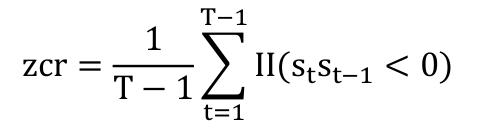
\includegraphics{zcr.png}
\caption{ZCR}
\end{figure}

Aqui exibimos o gráfico da ZCR sobreposto ao gráfico da forma de onda da
música. Como podemos ver, cada gênero, representado por uma canção,
apresenta uma curva própria no frame que utilizamos.

    \begin{Verbatim}[commandchars=\\\{\}]
{\color{incolor}In [{\color{incolor}4}]:} \PY{n}{plots}\PY{o}{.}\PY{n}{plot\PYZus{}superimprose\PYZus{}wave}\PY{p}{(}\PY{n}{waveform}\PY{p}{,} \PY{n}{SoundFeature}\PY{o}{.}\PY{n}{ZCR}\PY{p}{,}\PY{l+m+mi}{15}\PY{p}{)}
        \PY{n}{plots}\PY{o}{.}\PY{n}{plot\PYZus{}iqr}\PY{p}{(}\PY{n}{df}\PY{p}{,} \PY{n}{genres}\PY{p}{,} \PY{n}{SoundFeature}\PY{o}{.}\PY{n}{ZCR}\PY{p}{)}
\end{Verbatim}


    \begin{center}
    \adjustimage{max size={0.9\linewidth}{0.9\paperheight}}{output_10_0.png}
    \end{center}
    { \hspace*{\fill} \\}
    
    \begin{center}
    \adjustimage{max size={0.9\linewidth}{0.9\paperheight}}{output_10_1.png}
    \end{center}
    { \hspace*{\fill} \\}
    
    \textbf{2) Root mean square - RMS}: Indica a medida da onda de energia
num período de tempo, ou seja, o volume ou intensidade de uma faixa onde
pegamos um seus valores e calculamos a raiz quadrada da média ao quadro.
Aqui será utilizado para detectar as fronteiras entre sinais de fala e
música, ou a sonoridade da música. Está feature é definida pela seguinte
equação:

\begin{figure}[htbp]
\centering
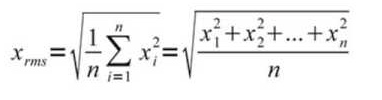
\includegraphics{rms.png}
\caption{RMS}
\end{figure}

Aqui exibimos o gráfico do RMS sobreposto ao gráfico da forma de onda da
música. Como podemos ver, cada gênero, representado por uma canção,
apresenta uma curva própria no frame que utilizamos.

    \begin{Verbatim}[commandchars=\\\{\}]
{\color{incolor}In [{\color{incolor}5}]:} \PY{n}{plots}\PY{o}{.}\PY{n}{plot\PYZus{}superimprose\PYZus{}wave}\PY{p}{(}\PY{n}{waveform}\PY{p}{,} \PY{n}{SoundFeature}\PY{o}{.}\PY{n}{RMS}\PY{p}{,}\PY{l+m+mi}{15}\PY{p}{)}
        \PY{n}{plots}\PY{o}{.}\PY{n}{plot\PYZus{}iqr}\PY{p}{(}\PY{n}{df}\PY{p}{,} \PY{n}{genres}\PY{p}{,} \PY{n}{SoundFeature}\PY{o}{.}\PY{n}{RMS}\PY{p}{)}
\end{Verbatim}


    \begin{center}
    \adjustimage{max size={0.9\linewidth}{0.9\paperheight}}{output_12_0.png}
    \end{center}
    { \hspace*{\fill} \\}
    
    \begin{center}
    \adjustimage{max size={0.9\linewidth}{0.9\paperheight}}{output_12_1.png}
    \end{center}
    { \hspace*{\fill} \\}
    
    \textbf{3) Spectrum Centroid - SC}:

Diferentemente das features anteriores, esta é um feature baseada na
frequência, que indica onde o ``centro de massa'' do espectro está
localizado e na prática costuma ser usado como medida do timbre musical.

Por ser uma medida no campo da frequência, acaba não sendo possível
visualizá-la de forma fácil apenas com os gráficos de onda da música,
principalmente quando as frequências são altas. Isto será visto mais
adiante, mas por hora vamos considerar que precisamos melhorar a forma
de capturar informações que estão "escondidas" no domínio da frequência.
Para superar esta dificuldade de conseguir informação de tempo no
domínio da frequência nós podemos utilizar a técnica chamada Short Time
Fourier Transform, ou STFT. O STFT divide a música em janelas curtas (na
ordem de milissegundos) e, em seguida, aplica a transformada de Fourier
de cada uma das janelas.

    \begin{Verbatim}[commandchars=\\\{\}]
{\color{incolor}In [{\color{incolor}6}]:} \PY{n}{plots}\PY{o}{.}\PY{n}{plot\PYZus{}superimprose\PYZus{}wave}\PY{p}{(}\PY{n}{waveform}\PY{p}{,} \PY{n}{SoundFeature}\PY{o}{.}\PY{n}{SC}\PY{p}{,}\PY{l+m+mi}{15}\PY{p}{)}
        \PY{n}{plots}\PY{o}{.}\PY{n}{plot\PYZus{}iqr}\PY{p}{(}\PY{n}{df}\PY{p}{,} \PY{n}{genres}\PY{p}{,} \PY{n}{SoundFeature}\PY{o}{.}\PY{n}{SC}\PY{p}{)}
\end{Verbatim}


    \begin{center}
    \adjustimage{max size={0.9\linewidth}{0.9\paperheight}}{output_14_0.png}
    \end{center}
    { \hspace*{\fill} \\}
    
    \begin{center}
    \adjustimage{max size={0.9\linewidth}{0.9\paperheight}}{output_14_1.png}
    \end{center}
    { \hspace*{\fill} \\}
    
    Como esta é uma feature que está no domínio da frequência, podemos
verificar através de espectrogramas como as frequências variam de acordo
com instrumentos utilizados. Por exemplo, a canção 3.wav utilizada no
gênero jazz, apresenta uma variação brusca no segundo 10, que coincide
com o momento em que o saxofone toca notas altas. Já o espectrograma do
gênero rock exibe vários picos de frequência ao longo da música, que
corresponde a batida da bateria, e também por volta do segudo 10 há um
aumento de frequência por alguns momentos, correspondendo a voz do
cantor que é "estendida" na música.

    \begin{Verbatim}[commandchars=\\\{\}]
{\color{incolor}In [{\color{incolor}7}]:} \PY{n}{plots}\PY{o}{.}\PY{n}{plot\PYZus{}spectrograms}\PY{p}{(}\PY{n}{waveform}\PY{p}{,} \PY{n}{duration}\PY{o}{=}\PY{l+m+mi}{20}\PY{p}{)}
\end{Verbatim}


    \begin{center}
    \adjustimage{max size={0.9\linewidth}{0.9\paperheight}}{output_16_0.png}
    \end{center}
    { \hspace*{\fill} \\}
    
    \textbf{4) Mel Frequency Cepstral Coefficients - MFCCs: Análise da
Feature}: Esta é uma feature classificada como psicoacústica, ou seja, é
baseada na percepção que o ser humano tem de perceber os sons. Essa
percepção humana do sons varia com a frequência e é representado aqui
através da Mel Scale Frequency, proposta por Stevens, Volkmann, and
Newman em 1937{[}8{]}. Esta escala é baseada em um mapeamento entre
frequência real e o "pitch" aparentemente percebido pelo ouvido humano.
Em frequências baixas a escala é linear, porém conforme a frequência
sobe o ouvido humano passa a ter mais dificuldade na percepção dos sons,
ou seja, somos mais sensíveis às baixas frequências e menos sensíveis às
altas frequências.

\begin{figure}[htbp]
\centering
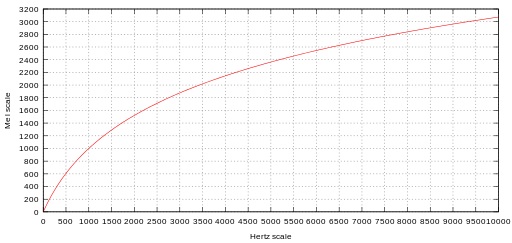
\includegraphics{Mel-Hz_plot.svg.png}
\caption{Escala MEL}
\end{figure}

Esta feature tem sido muito popular no campo do reconhecimento de fala.
Neste trabalho não iremos nos aprofundar os mecanismo de extração dessa
feature, uma vez que a biblioteca librosa faz esse trabalho. No entanto,
o algoritmo básico de extração dessa feature é mostrado abaixo:

\begin{figure}[htbp]
\centering
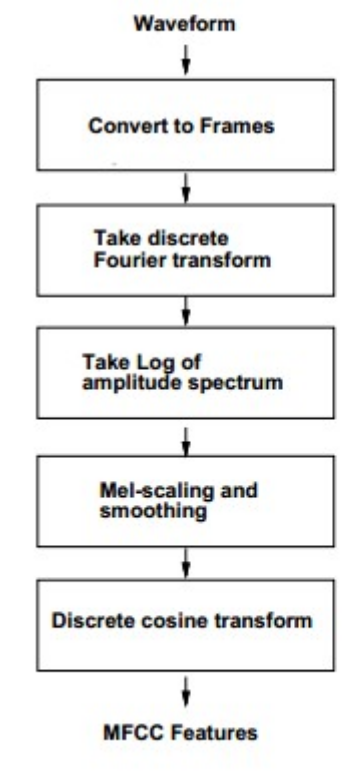
\includegraphics{mfccs.png}
\caption{MFCCS\_FEATURE}
\end{figure}

Neste ponto iremos extrair 13 bandas MCFFs juntamente com seu valor
delta, que representa a estimativa local da derivada dos dados de
entrada ao longo tempo, em outras palavras, o delta representa a
variação de coeficiente entre frames. Este valores são as divisões de
bandas de frequência na escala Mel. Poderíamos dividir em mais ou menos
bandas, no entanto, as bandas muito altas representam mudanças rápidas
no banco de filtros MEL e degradam a performance ASR{[}9{]}, por isso as
desconsideramos.

    \subsubsection{Benchmark}\label{benchmark}

No estudo realizado por Seyerlehner et al{[}7{]}, é mencionado pelo
autor que até o momento somente um trabalho publicado trata de comparar
a classificação musical realizada por humanos com a classificação
realizada de forma automática por computadores. O trabalho que realizou
esse experimento foi publicado por Tzanetakis et al {[}1{]}. Neste
estudo foram classificadas 190 músicas em 19 diferentes categorias. A
classificação humana apresentou acurácia entre 26\% e 71\%, com uma
média de 55\%. Para o nosso trabalho iremos considerar um objetivo de
70\% já que iremos trabalhar com um conjunto reduzido de apenas 5
gêneros musicais.

\subsection{III. Metodologia}\label{iii.-metodologia}

\subsubsection{Pré-processamento de
dados}\label{pruxe9-processamento-de-dados}

Como mencionado anteriormente, iremos trabalhar com 4 features
distintas. Do domínio do tempo temos Zero-Crossing Rate e a Root Mean
Square, do domínio da frequência temos a Spectral Centroid e do domínio
espectral mas filtrados em Mel Frequency Banks, que são bancos de
atributos divididos na escala de frequência Mel, a feature Mel Frequency
Cepstral Coefficients.

A extração das features é realizada pela biblioteca librosa, através da
funções \emph{zero\_crossing\_rate, rmse, spectral\_centroid e mfcc}.
Este valores são armazenados em um dataframe para o posterior uso. Cada
amostra contém 330.0750 valores (22050 Hz x 15 seg.).

A feature MFCC está sendo tratada como um banco de atributos da escala
Mel, este banco está divido em treze bandas, então ela será desdobrada
em treze features.

Para combinar a informação de todos as bandas e coeficientes, nós iremos
calcular suas médias e desvios padrões. Eliminaremos o MFCC do índice
zero, pois não agrega informação. Assim teremos um total de 58 features
(zcr std, zcr mean, rms std, rms mean, sc std, sc mean, 12 x MFCCs std e
12 x MFCCs mean, 12 x MFCCs delta std e 12 x MFCCs delta mean) mais a
categoria do gênero musical.

    \begin{Verbatim}[commandchars=\\\{\}]
{\color{incolor}In [{\color{incolor}6}]:} \PY{n}{features}\PY{p}{,} \PY{n}{labels}\PY{p}{,} \PY{n}{X}\PY{p}{,} \PY{n}{y} \PY{o}{=} \PY{n}{npdata}\PY{o}{.}\PY{n}{prepare\PYZus{}data}\PY{p}{(}\PY{n}{df}\PY{p}{)}
\end{Verbatim}


    Após a extração das features, podemos visualizar a correlação entre
elas.

    \begin{Verbatim}[commandchars=\\\{\}]
{\color{incolor}In [{\color{incolor}7}]:} \PY{n}{title}\PY{o}{=}\PY{l+s+s1}{\PYZsq{}}\PY{l+s+s1}{Correlation matrix}\PY{l+s+s1}{\PYZsq{}}
        
        \PY{n}{plt}\PY{o}{.}\PY{n}{figure}\PY{p}{(}\PY{n}{figsize}\PY{o}{=}\PY{p}{(}\PY{l+m+mi}{14}\PY{p}{,} \PY{l+m+mi}{10}\PY{p}{)}\PY{p}{)}
        \PY{n}{sns}\PY{o}{.}\PY{n}{heatmap}\PY{p}{(}\PY{n}{X}\PY{o}{.}\PY{n}{corr}\PY{p}{(}\PY{p}{)}\PY{p}{,} \PY{n}{annot}\PY{o}{=}\PY{k+kc}{False}\PY{p}{,} \PY{n}{cmap}\PY{o}{=}\PY{n}{plt}\PY{o}{.}\PY{n}{cm}\PY{o}{.}\PY{n}{coolwarm}\PY{p}{)}
        \PY{n}{plt}\PY{o}{.}\PY{n}{yticks}\PY{p}{(}\PY{n}{rotation}\PY{o}{=}\PY{l+m+mi}{0}\PY{p}{,} \PY{n}{fontsize}\PY{o}{=}\PY{l+m+mi}{8}\PY{p}{)}
        \PY{n}{plt}\PY{o}{.}\PY{n}{xticks}\PY{p}{(}\PY{n}{rotation}\PY{o}{=}\PY{l+m+mi}{90}\PY{p}{,} \PY{n}{fontsize}\PY{o}{=}\PY{l+m+mi}{8}\PY{p}{)}
        \PY{n}{plt}\PY{o}{.}\PY{n}{title}\PY{p}{(}\PY{n}{title}\PY{p}{)}
        \PY{n}{plt}\PY{o}{.}\PY{n}{savefig}\PY{p}{(}\PY{l+s+s1}{\PYZsq{}}\PY{l+s+s1}{corr\PYZus{}matrix.png}\PY{l+s+s1}{\PYZsq{}}\PY{p}{)}
\end{Verbatim}


    \begin{center}
    \adjustimage{max size={0.9\linewidth}{0.9\paperheight}}{output_21_0.png}
    \end{center}
    { \hspace*{\fill} \\}
    
    Podemos notar que as features ZCR, RMS e SC são bem correlacionadas
entre si, enquanto as features MFCCs exibem correlações variadas.

    \subsubsection{Implementação}\label{implementauxe7uxe3o}

Uma vez que temos as features extraídas e pré-processadas, iremos de
fato submeter nossos dados ao modelo de treinamento. Para isto usaremos
o k-NN.

K-NN é modelo de aprendizagem baseado em instâncias para classificar
diferentes classes de dados. A ideia do KNN é descobrir qual classe tem
mais pontos próximos aos dados do teste. Escolhe um k específico que
significa encontrar k vizinhos. Ele simplesmente armazena os dados e o
rótulo memória e uma vez se peça para classificar uma instância
particular, calcula a distância (com função de distância específica) a
todos os pontos nos dados de treinamento e atribui um rótulo de acordo
com o rótulo dos vizinhos K mais próximos. A razão para escolha deste
algoritmo é sua simplicidade e por ser bem conhecido no uso de
reconhecimento de padrões, para uso em problemas de classificação
supervisionada. No entanto, por ser sensível aos dados, ele requer um
bom conjunto de features para que possa performar de forma satisfatória,
e para isso precisaremos fazer alguma normalização dos dados antes do
treinamento. Antes de utilizá-lo ainda precisamos normalizar os dados

    \begin{Verbatim}[commandchars=\\\{\}]
{\color{incolor}In [{\color{incolor}9}]:} \PY{k+kn}{from} \PY{n+nn}{sklearn}\PY{n+nn}{.}\PY{n+nn}{preprocessing} \PY{k}{import} \PY{n}{normalize}\PY{p}{,} \PY{n}{StandardScaler}\PY{p}{,} \PY{n}{RobustScaler}
        
        \PY{n}{scaler} \PY{o}{=} \PY{n}{StandardScaler}\PY{p}{(}\PY{p}{)}
        \PY{n}{X\PYZus{}normal} \PY{o}{=} \PY{n}{scaler}\PY{o}{.}\PY{n}{fit\PYZus{}transform}\PY{p}{(}\PY{n}{X}\PY{p}{)}
        \PY{n}{X\PYZus{}normal} \PY{o}{=} \PY{n}{pd}\PY{o}{.}\PY{n}{DataFrame}\PY{p}{(}\PY{n}{X\PYZus{}normal}\PY{p}{,} \PY{n}{columns}\PY{o}{=}\PY{n}{X}\PY{o}{.}\PY{n}{columns}\PY{p}{)}
\end{Verbatim}


    \paragraph{Detecção de valores atípicos
(Outlier)}\label{detecuxe7uxe3o-de-valores-atuxedpicos-outlier}

Para evitar que dados discrepantes possam enviesar os resultados,
aplicamos o Método Turco para identificar outliers: Um passo do
discrepante é calculado 1,5 vezes a variação interquartil (IQR). Um
ponto de dados com um atributo que está além de um passo de um
discrepante do IQR para aquele atributo, ele será considerado anormal. E
removeremos os outliers que estiverem duplicados em mais de uma features

    \begin{Verbatim}[commandchars=\\\{\}]
{\color{incolor}In [{\color{incolor}18}]:} \PY{k+kn}{import} \PY{n+nn}{itertools}
         
         \PY{n}{outliers\PYZus{}lst} \PY{o}{=} \PY{p}{[}\PY{p}{]}
         
         \PY{k}{for} \PY{n}{feature} \PY{o+ow}{in} \PY{n}{X\PYZus{}normal}\PY{o}{.}\PY{n}{keys}\PY{p}{(}\PY{p}{)}\PY{p}{:}
             
             \PY{n}{Q1} \PY{o}{=} \PY{n}{np}\PY{o}{.}\PY{n}{percentile}\PY{p}{(}\PY{n}{X\PYZus{}normal}\PY{p}{[}\PY{n}{feature}\PY{p}{]}\PY{p}{,} \PY{l+m+mi}{25}\PY{p}{)}    
             \PY{n}{Q3} \PY{o}{=} \PY{n}{np}\PY{o}{.}\PY{n}{percentile}\PY{p}{(}\PY{n}{X\PYZus{}normal}\PY{p}{[}\PY{n}{feature}\PY{p}{]}\PY{p}{,} \PY{l+m+mi}{75}\PY{p}{)}
             
             \PY{n}{step} \PY{o}{=} \PY{l+m+mf}{1.5} \PY{o}{*} \PY{p}{(}\PY{n}{Q3}\PY{o}{\PYZhy{}}\PY{n}{Q1}\PY{p}{)}
             
             \PY{n}{r\PYZus{}outlier} \PY{o}{=} \PY{n}{X\PYZus{}normal}\PY{p}{[}\PY{o}{\PYZti{}}\PY{p}{(}\PY{p}{(}\PY{n}{X\PYZus{}normal}\PY{p}{[}\PY{n}{feature}\PY{p}{]} \PY{o}{\PYZgt{}}\PY{o}{=} \PY{n}{Q1} \PY{o}{\PYZhy{}} \PY{n}{step}\PY{p}{)} \PY{o}{\PYZam{}} \PY{p}{(}\PY{n}{X\PYZus{}normal}\PY{p}{[}\PY{n}{feature}\PY{p}{]} \PY{o}{\PYZlt{}}\PY{o}{=} \PY{n}{Q3} \PY{o}{+} \PY{n}{step}\PY{p}{)}\PY{p}{)}\PY{p}{]}
             
             \PY{n}{outliers\PYZus{}lst}\PY{o}{.}\PY{n}{append}\PY{p}{(}\PY{n+nb}{list}\PY{p}{(}\PY{n}{r\PYZus{}outlier}\PY{o}{.}\PY{n}{index}\PY{p}{)}\PY{p}{)}
                 
         \PY{n}{outliers} \PY{o}{=} \PY{n+nb}{list}\PY{p}{(}\PY{n}{itertools}\PY{o}{.}\PY{n}{chain}\PY{o}{.}\PY{n}{from\PYZus{}iterable}\PY{p}{(}\PY{n}{outliers\PYZus{}lst}\PY{p}{)}\PY{p}{)}
         
         \PY{n}{uniq\PYZus{}outliers} \PY{o}{=} \PY{n+nb}{list}\PY{p}{(}\PY{n+nb}{set}\PY{p}{(}\PY{n}{outliers}\PY{p}{)}\PY{p}{)}    
         
         \PY{n+nb}{print}\PY{p}{(} \PY{l+s+s1}{\PYZsq{}}\PY{l+s+s1}{Unique list:}\PY{l+s+se}{\PYZbs{}n}\PY{l+s+s1}{\PYZsq{}}\PY{p}{,} \PY{n}{uniq\PYZus{}outliers}\PY{p}{)}
         
         \PY{n}{X\PYZus{}normal} \PY{o}{=} \PY{n}{X\PYZus{}normal}\PY{o}{.}\PY{n}{drop}\PY{p}{(}\PY{n}{X\PYZus{}normal}\PY{o}{.}\PY{n}{index}\PY{p}{[}\PY{n}{uniq\PYZus{}outliers}\PY{p}{]}\PY{p}{)}\PY{o}{.}\PY{n}{reset\PYZus{}index}\PY{p}{(}\PY{n}{drop} \PY{o}{=} \PY{k+kc}{True}\PY{p}{)}
         \PY{n}{y} \PY{o}{=} \PY{n}{y}\PY{o}{.}\PY{n}{drop}\PY{p}{(}\PY{n}{y}\PY{o}{.}\PY{n}{index}\PY{p}{[}\PY{n}{uniq\PYZus{}outliers}\PY{p}{]}\PY{p}{)}\PY{o}{.}\PY{n}{reset\PYZus{}index}\PY{p}{(}\PY{n}{drop} \PY{o}{=} \PY{k+kc}{True}\PY{p}{)}
\end{Verbatim}


    \begin{Verbatim}[commandchars=\\\{\}]
Unique list:
 [1, 6, 9, 12, 31, 45, 47, 59, 70, 74, 92, 97, 99, 102, 103, 114, 115, 116, 117, 118, 124, 125, 127, 128, 130, 131, 132, 133, 134, 135, 136, 137, 143, 144, 145, 147, 150, 152, 153, 154, 156, 157, 159, 160, 164, 166, 167, 168, 172, 176, 177, 178, 180, 184, 186, 192, 194, 199, 204, 208, 209, 212, 215, 216, 217, 220, 224, 225, 227, 233, 236, 239, 240, 242, 243, 247, 252, 260, 262, 264, 265, 266, 267, 268, 272, 273, 275, 278, 279, 280, 282, 283, 284, 288, 289, 290, 291, 293, 298, 299, 302, 304, 305, 310, 313, 314, 316, 317, 320, 321, 322, 323, 324, 325, 326, 328, 329, 330, 331, 334, 338, 341, 342, 344, 345, 346, 351, 352, 354, 355, 357, 360, 361, 362, 363, 365, 366, 367, 368, 370, 373, 376, 380, 382, 383, 386, 387, 389, 390, 392, 393, 394, 395, 396, 400, 406, 408, 410, 432, 433, 435, 440, 446, 452, 453, 454, 459, 465, 467, 469, 472, 476, 486, 488, 489, 494, 495]

    \end{Verbatim}

    \subsubsection{k-Nearest Neighbors}\label{k-nearest-neighbors}

Uma vez que os dados tenham sido normalizados, iremos dividí-los em
conjunto de treinamento e teste. Porém alguns problemas de classificação
podem exibir um grande desequilíbrio na distribuição das classes-alvo:
por exemplo, pode haver várias vezes mais amostras negativas do que
amostras positivas. Nesses casos, recomenda-se usar amostragem
estratificada, e para isso, o sklearn implementa a função
StratifiedShuffleSplit, assim garantimos que as frequências de classe
relativas sejam aproximadamente preservadas.

    \begin{Verbatim}[commandchars=\\\{\}]
{\color{incolor}In [{\color{incolor}92}]:} \PY{n}{sss} \PY{o}{=} \PY{n}{StratifiedShuffleSplit}\PY{p}{(}\PY{n}{n\PYZus{}splits}\PY{o}{=}\PY{l+m+mi}{10}\PY{p}{,} \PY{n}{test\PYZus{}size}\PY{o}{=}\PY{l+m+mf}{0.25}\PY{p}{,} \PY{n}{random\PYZus{}state}\PY{o}{=}\PY{l+m+mi}{4}\PY{p}{)}
         \PY{n}{accuracies} \PY{o}{=} \PY{p}{[}\PY{p}{]}
         \PY{k}{for} \PY{n}{train\PYZus{}index}\PY{p}{,} \PY{n}{test\PYZus{}index} \PY{o+ow}{in} \PY{n}{sss}\PY{o}{.}\PY{n}{split}\PY{p}{(}\PY{n}{X\PYZus{}normal}\PY{p}{,} \PY{n}{y}\PY{p}{)}\PY{p}{:}
             \PY{n}{X\PYZus{}train}\PY{p}{,} \PY{n}{X\PYZus{}test} \PY{o}{=} \PY{n}{X\PYZus{}normal}\PY{o}{.}\PY{n}{iloc}\PY{p}{[}\PY{n}{train\PYZus{}index}\PY{p}{]}\PY{p}{,} \PY{n}{X\PYZus{}normal}\PY{o}{.}\PY{n}{iloc}\PY{p}{[}\PY{n}{test\PYZus{}index}\PY{p}{]}
             \PY{n}{y\PYZus{}train}\PY{p}{,} \PY{n}{y\PYZus{}test} \PY{o}{=} \PY{n}{y}\PY{p}{[}\PY{n}{train\PYZus{}index}\PY{p}{]}\PY{p}{,} \PY{n}{y}\PY{p}{[}\PY{n}{test\PYZus{}index}\PY{p}{]}
         
             \PY{n}{classifier} \PY{o}{=} \PY{n}{KNeighborsClassifier}\PY{p}{(}\PY{n}{n\PYZus{}neighbors}\PY{o}{=}\PY{l+m+mi}{1}\PY{p}{)}
             \PY{n}{classifier}\PY{o}{.}\PY{n}{fit}\PY{p}{(}\PY{n}{X\PYZus{}train}\PY{p}{,} \PY{n}{y\PYZus{}train}\PY{p}{)}
         
             \PY{n}{y\PYZus{}preds} \PY{o}{=} \PY{n}{classifier}\PY{o}{.}\PY{n}{predict}\PY{p}{(}\PY{n}{X\PYZus{}test}\PY{p}{)}
         
             \PY{n}{accuracies}\PY{o}{.}\PY{n}{append}\PY{p}{(}\PY{n}{accuracy\PYZus{}score}\PY{p}{(}\PY{n}{y\PYZus{}test}\PY{p}{,} \PY{n}{y\PYZus{}preds}\PY{p}{)}\PY{p}{)}
         
         \PY{n+nb}{print}\PY{p}{(}\PY{n}{f}\PY{l+s+s1}{\PYZsq{}}\PY{l+s+s1}{Acurácia média: }\PY{l+s+s1}{\PYZob{}}\PY{l+s+s1}{np.round(np.mean(accuracies),3):.2}\PY{l+s+s1}{\PYZpc{}}\PY{l+s+s1}{\PYZcb{}}\PY{l+s+s1}{\PYZsq{}}\PY{p}{)}
\end{Verbatim}


    \begin{Verbatim}[commandchars=\\\{\}]
Acurácia média: 73.30\%

    \end{Verbatim}

    O valor médio obtido para a acurácia foi de 73,30\%. Neste treinamento
usamos k igual a 1, no entanto, podemos tentar melhorar esse percentual
manipulando alguns parâmetros do k-NN.

\subsubsection{Refinamento}\label{refinamento}

A fim de tentar melhorar a performance do nosso algoritmo, iremos
aplicar a técnica conhecida como GridSearch que para o nosso caso
consistirá em aplicar o k-NN repetidas vezes utilizando diferentes
valores para k. Para isso, precisamos especificar quais valores de k
queremos, também iremos especificar outros dois parâmetros:

\emph{weights}: quando temos distribuições de classe distorcidas pode-se
usar uma votação ponderada. A classe de cada um dos vizinhos K é
multiplicada por um peso proporcional ao inverso da distância desse
ponto ao ponto de teste dado. Isso garante que os vizinhos mais próximos
contribuam mais para a votação final do que os mais distantes. No
sklearn isso é feito especificando esse parâmetro para "distance". Já o
parâmetro com o valor "uninform" faz o k-NN ter o comportamento padrão

\emph{p}: este parâmetro especifica que tipo de métrica de distância
será tomada pelo algoritimo. No sklearn, utilizaremos o
\emph{manhattan\_distance} e o \emph{euclidean\_distance}

    \begin{Verbatim}[commandchars=\\\{\}]
{\color{incolor}In [{\color{incolor}30}]:} \PY{n}{k}\PY{o}{=}\PY{l+m+mi}{20}
         
         \PY{n}{sss} \PY{o}{=} \PY{n}{StratifiedShuffleSplit}\PY{p}{(}\PY{n}{n\PYZus{}splits}\PY{o}{=}\PY{l+m+mi}{10}\PY{p}{,} \PY{n}{test\PYZus{}size}\PY{o}{=}\PY{l+m+mf}{0.25}\PY{p}{,} \PY{n}{random\PYZus{}state}\PY{o}{=}\PY{l+m+mi}{4}\PY{p}{)}
         \PY{n}{accuracies} \PY{o}{=} \PY{p}{[}\PY{p}{]}
         
         \PY{n}{result\PYZus{}test}\PY{o}{=}\PY{n}{np}\PY{o}{.}\PY{n}{zeros}\PY{p}{(}\PY{n}{k}\PY{p}{)}
         \PY{n}{result\PYZus{}train}\PY{o}{=}\PY{n}{np}\PY{o}{.}\PY{n}{zeros}\PY{p}{(}\PY{n}{k}\PY{p}{)}
         
         \PY{k}{for} \PY{n}{k1} \PY{o+ow}{in} \PY{n+nb}{range}\PY{p}{(}\PY{l+m+mi}{1}\PY{p}{,} \PY{n}{k}\PY{p}{)}\PY{p}{:}
             \PY{n}{acc\PYZus{}train}\PY{o}{=}\PY{l+m+mi}{0}
             \PY{n}{acc\PYZus{}test}\PY{o}{=}\PY{l+m+mi}{0}
             \PY{k}{for} \PY{n}{train\PYZus{}index}\PY{p}{,} \PY{n}{test\PYZus{}index} \PY{o+ow}{in} \PY{n}{sss}\PY{o}{.}\PY{n}{split}\PY{p}{(}\PY{n}{X\PYZus{}normal}\PY{p}{,} \PY{n}{y}\PY{p}{)}\PY{p}{:}
                 \PY{n}{X\PYZus{}train}\PY{p}{,} \PY{n}{X\PYZus{}test} \PY{o}{=} \PY{n}{X\PYZus{}normal}\PY{o}{.}\PY{n}{iloc}\PY{p}{[}\PY{n}{train\PYZus{}index}\PY{p}{]}\PY{p}{,} \PY{n}{X\PYZus{}normal}\PY{o}{.}\PY{n}{iloc}\PY{p}{[}\PY{n}{test\PYZus{}index}\PY{p}{]}
                 \PY{n}{y\PYZus{}train}\PY{p}{,} \PY{n}{y\PYZus{}test} \PY{o}{=} \PY{n}{y}\PY{p}{[}\PY{n}{train\PYZus{}index}\PY{p}{]}\PY{p}{,} \PY{n}{y}\PY{p}{[}\PY{n}{test\PYZus{}index}\PY{p}{]}
         
                 \PY{n}{classifier} \PY{o}{=} \PY{n}{KNeighborsClassifier}\PY{p}{(}\PY{n}{n\PYZus{}neighbors}\PY{o}{=}\PY{n}{k1}\PY{p}{)}
                 \PY{n}{classifier}\PY{o}{.}\PY{n}{fit}\PY{p}{(}\PY{n}{X\PYZus{}train}\PY{p}{,} \PY{n}{y\PYZus{}train}\PY{p}{)}
         
                 \PY{n}{y\PYZus{}pred\PYZus{}train}\PY{o}{=}\PY{n}{classifier}\PY{o}{.}\PY{n}{predict}\PY{p}{(}\PY{n}{X\PYZus{}train}\PY{p}{)}
                 \PY{n}{y\PYZus{}pred\PYZus{}test}\PY{o}{=}\PY{n}{classifier}\PY{o}{.}\PY{n}{predict}\PY{p}{(}\PY{n}{X\PYZus{}test}\PY{p}{)}
         
                 \PY{n}{acc\PYZus{}train}\PY{o}{+}\PY{o}{=}\PY{n}{accuracy\PYZus{}score}\PY{p}{(}\PY{n}{y\PYZus{}train}\PY{p}{,}\PY{n}{y\PYZus{}pred\PYZus{}train}\PY{p}{)}
                 \PY{n}{acc\PYZus{}test}\PY{o}{+}\PY{o}{=}\PY{n}{accuracy\PYZus{}score}\PY{p}{(}\PY{n}{y\PYZus{}test}\PY{p}{,}\PY{n}{y\PYZus{}pred\PYZus{}test}\PY{p}{)}
         
             \PY{n}{result\PYZus{}train}\PY{p}{[}\PY{n}{k1}\PY{o}{\PYZhy{}}\PY{l+m+mi}{1}\PY{p}{]}\PY{o}{=}\PY{n}{acc\PYZus{}train}\PY{o}{/}\PY{l+m+mi}{10}
             \PY{n}{result\PYZus{}test}\PY{p}{[}\PY{n}{k1}\PY{o}{\PYZhy{}}\PY{l+m+mi}{1}\PY{p}{]}\PY{o}{=}\PY{n}{acc\PYZus{}test}\PY{o}{/}\PY{l+m+mi}{10}
         
         \PY{n}{fig}\PY{p}{,}\PY{n}{ax}\PY{o}{=}\PY{n}{plt}\PY{o}{.}\PY{n}{subplots}\PY{p}{(}\PY{n}{figsize}\PY{o}{=}\PY{p}{(}\PY{l+m+mi}{10}\PY{p}{,}\PY{l+m+mi}{7}\PY{p}{)}\PY{p}{)}
         \PY{n}{plt}\PY{o}{.}\PY{n}{plot}\PY{p}{(}\PY{n}{result\PYZus{}train}\PY{p}{,}\PY{l+s+s1}{\PYZsq{}}\PY{l+s+s1}{ro\PYZhy{}}\PY{l+s+s1}{\PYZsq{}}\PY{p}{,}\PY{n}{label}\PY{o}{=}\PY{l+s+s1}{\PYZsq{}}\PY{l+s+s1}{training}\PY{l+s+s1}{\PYZsq{}}\PY{p}{)}
         \PY{n}{plt}\PY{o}{.}\PY{n}{plot}\PY{p}{(}\PY{n}{result\PYZus{}test}\PY{p}{,}\PY{l+s+s1}{\PYZsq{}}\PY{l+s+s1}{bo\PYZhy{}}\PY{l+s+s1}{\PYZsq{}}\PY{p}{,}\PY{n}{label}\PY{o}{=}\PY{l+s+s1}{\PYZsq{}}\PY{l+s+s1}{validation}\PY{l+s+s1}{\PYZsq{}}\PY{p}{)}
         \PY{n}{plt}\PY{o}{.}\PY{n}{ylabel}\PY{p}{(}\PY{l+s+s1}{\PYZsq{}}\PY{l+s+s1}{Accuracy}\PY{l+s+s1}{\PYZsq{}}\PY{p}{)}
         \PY{n}{plt}\PY{o}{.}\PY{n}{title}\PY{p}{(}\PY{l+s+s1}{\PYZsq{}}\PY{l+s+s1}{Trining, validation result for k selection}\PY{l+s+s1}{\PYZsq{}}\PY{p}{)}
         \PY{n}{plt}\PY{o}{.}\PY{n}{xlabel}\PY{p}{(}\PY{l+s+s1}{\PYZsq{}}\PY{l+s+s1}{k }\PY{l+s+se}{\PYZbs{}n}\PY{l+s+s1}{ longitude}\PY{l+s+s1}{\PYZsq{}}\PY{p}{)}
         \PY{n}{ax}\PY{o}{.}\PY{n}{legend}\PY{p}{(}\PY{n}{loc}\PY{o}{=}\PY{l+s+s1}{\PYZsq{}}\PY{l+s+s1}{best}\PY{l+s+s1}{\PYZsq{}}\PY{p}{,} \PY{n}{prop}\PY{o}{=}\PY{p}{\PYZob{}}\PY{l+s+s1}{\PYZsq{}}\PY{l+s+s1}{size}\PY{l+s+s1}{\PYZsq{}}\PY{p}{:}\PY{l+s+s1}{\PYZsq{}}\PY{l+s+s1}{small}\PY{l+s+s1}{\PYZsq{}}\PY{p}{\PYZcb{}}\PY{p}{)}
\end{Verbatim}


\begin{Verbatim}[commandchars=\\\{\}]
{\color{outcolor}Out[{\color{outcolor}30}]:} <matplotlib.legend.Legend at 0x7f6bf0bbb780>
\end{Verbatim}
            
    \begin{center}
    \adjustimage{max size={0.9\linewidth}{0.9\paperheight}}{output_30_1.png}
    \end{center}
    { \hspace*{\fill} \\}
    
    \begin{Verbatim}[commandchars=\\\{\}]
{\color{incolor}In [{\color{incolor}19}]:} \PY{n}{parameters} \PY{o}{=} \PY{p}{\PYZob{}}\PY{l+s+s1}{\PYZsq{}}\PY{l+s+s1}{n\PYZus{}neighbors}\PY{l+s+s1}{\PYZsq{}}\PY{p}{:}\PY{n}{np}\PY{o}{.}\PY{n}{arange}\PY{p}{(}\PY{l+m+mi}{1}\PY{p}{,}\PY{l+m+mi}{10}\PY{p}{,}\PY{l+m+mi}{1}\PY{p}{)}\PY{p}{,}
                       \PY{l+s+s1}{\PYZsq{}}\PY{l+s+s1}{weights}\PY{l+s+s1}{\PYZsq{}}\PY{p}{:}\PY{p}{[}\PY{l+s+s1}{\PYZsq{}}\PY{l+s+s1}{uniform}\PY{l+s+s1}{\PYZsq{}}\PY{p}{,}\PY{l+s+s1}{\PYZsq{}}\PY{l+s+s1}{distance}\PY{l+s+s1}{\PYZsq{}}\PY{p}{]}\PY{p}{,}
                       \PY{l+s+s1}{\PYZsq{}}\PY{l+s+s1}{p}\PY{l+s+s1}{\PYZsq{}}\PY{p}{:}\PY{p}{[}\PY{l+m+mi}{1}\PY{p}{,}\PY{l+m+mi}{2}\PY{p}{]}\PY{p}{\PYZcb{}}
         
         \PY{n}{X\PYZus{}train}\PY{p}{,} \PY{n}{X\PYZus{}test}\PY{p}{,} \PY{n}{y\PYZus{}train}\PY{p}{,} \PY{n}{y\PYZus{}test} \PY{o}{=} \PY{n}{train\PYZus{}test\PYZus{}split}\PY{p}{(}\PY{n}{X\PYZus{}normal}\PY{p}{,} \PY{n}{y}\PY{p}{,} \PY{n}{test\PYZus{}size}\PY{o}{=}\PY{l+m+mf}{0.25}\PY{p}{,} \PY{n}{random\PYZus{}state}\PY{o}{=}\PY{l+m+mi}{0}\PY{p}{)}
         
         \PY{n}{sss} \PY{o}{=} \PY{n}{StratifiedShuffleSplit}\PY{p}{(}\PY{n}{n\PYZus{}splits}\PY{o}{=}\PY{l+m+mi}{10}\PY{p}{,} \PY{n}{test\PYZus{}size}\PY{o}{=}\PY{l+m+mf}{0.25}\PY{p}{,} \PY{n}{random\PYZus{}state}\PY{o}{=}\PY{l+m+mi}{4}\PY{p}{,} \PY{p}{)}
         
         
         \PY{n}{grid} \PY{o}{=} \PY{n}{GridSearchCV}\PY{p}{(}\PY{n}{KNeighborsClassifier}\PY{p}{(}\PY{p}{)}\PY{p}{,} \PY{n}{parameters}\PY{p}{,} \PY{n}{cv}\PY{o}{=}\PY{n}{sss}\PY{p}{,} \PY{n}{scoring}\PY{o}{=}\PY{l+s+s1}{\PYZsq{}}\PY{l+s+s1}{accuracy}\PY{l+s+s1}{\PYZsq{}}\PY{p}{)}
         \PY{n}{grid}\PY{o}{.}\PY{n}{fit}\PY{p}{(}\PY{n}{X\PYZus{}train}\PY{p}{,} \PY{n}{y\PYZus{}train}\PY{p}{)}
         
         \PY{n+nb}{print}\PY{p}{(}\PY{n}{f}\PY{l+s+s1}{\PYZsq{}}\PY{l+s+s1}{Best score }\PY{l+s+si}{\PYZob{}grid.best\PYZus{}score\PYZus{}:.2\PYZpc{}\PYZcb{}}\PY{l+s+s1}{\PYZsq{}}\PY{p}{)}
         \PY{n+nb}{print}\PY{p}{(}\PY{n}{f}\PY{l+s+s1}{\PYZsq{}}\PY{l+s+s1}{Best params: }\PY{l+s+si}{\PYZob{}grid.best\PYZus{}params\PYZus{}\PYZcb{}}\PY{l+s+s1}{\PYZsq{}}\PY{p}{)}
         
         \PY{n}{y\PYZus{}pred} \PY{o}{=} \PY{n}{grid}\PY{o}{.}\PY{n}{predict}\PY{p}{(}\PY{n}{X\PYZus{}test}\PY{p}{)}
         
         \PY{n+nb}{print}\PY{p}{(}\PY{n}{classification\PYZus{}report}\PY{p}{(}\PY{n}{y\PYZus{}test}\PY{p}{,} \PY{n}{y\PYZus{}pred}\PY{p}{)}\PY{p}{)}
\end{Verbatim}


    \begin{Verbatim}[commandchars=\\\{\}]
Best score 78.52\%
Best params: \{'n\_neighbors': 3, 'p': 1, 'weights': 'distance'\}
             precision    recall  f1-score   support

      blues       0.73      0.57      0.64        14
  classical       0.88      0.83      0.86        18
       jazz       0.39      0.58      0.47        12
        pop       0.83      0.91      0.87        11
       rock       0.61      0.54      0.57        26

avg / total       0.69      0.67      0.67        81


    \end{Verbatim}

    Após a aplicação do GridSearchCV, conseguimos obter o valor de k=3 o
melhor resultado, elevando a pontuação para 78,52\% de acurácia. O
gráfico acima exibe o comportamento do treinamento e teste ao variar o
valor de k.

    \subsubsection{Bagging}\label{bagging}

Após a extração das features chegamos a um número significativo de
dimensões, portanto iremos utilizar o método de random subspaces aliado
ao Knn, isto é, vários modelos de Knn, cada um treinado num subconjunto
dos dados. Pra conseguirmos isto, utlizaremos o Bagging do sklearn, onde
controlaremos o max\_features e utilizaremos o knn como o
'base\_estimator' do Bagging.

    \begin{Verbatim}[commandchars=\\\{\}]
{\color{incolor}In [{\color{incolor}13}]:} \PY{k+kn}{from} \PY{n+nn}{sklearn}\PY{n+nn}{.}\PY{n+nn}{ensemble} \PY{k}{import} \PY{n}{BaggingClassifier}
         
         \PY{n}{knn} \PY{o}{=} \PY{n}{KNeighborsClassifier}\PY{p}{(}\PY{p}{)}
         \PY{n}{bagging} \PY{o}{=} \PY{n}{BaggingClassifier}\PY{p}{(}\PY{n}{knn}\PY{p}{,} \PY{n}{max\PYZus{}samples}\PY{o}{=}\PY{l+m+mf}{0.75}\PY{p}{,} \PY{n}{max\PYZus{}features}\PY{o}{=}\PY{o}{.}\PY{l+m+mi}{5}\PY{p}{)}
         
         \PY{n}{bagging\PYZus{}score} \PY{o}{=} \PY{n}{cross\PYZus{}val\PYZus{}score}\PY{p}{(}\PY{n}{bagging}\PY{p}{,} \PY{n}{X\PYZus{}normal}\PY{p}{,} \PY{n}{y}\PY{p}{,} \PY{n}{cv}\PY{o}{=}\PY{l+m+mi}{10}\PY{p}{,} \PY{n}{n\PYZus{}jobs}\PY{o}{=}\PY{o}{\PYZhy{}}\PY{l+m+mi}{1}\PY{p}{,} \PY{n}{scoring}\PY{o}{=}\PY{l+s+s1}{\PYZsq{}}\PY{l+s+s1}{accuracy}\PY{l+s+s1}{\PYZsq{}}\PY{p}{)}\PY{o}{.}\PY{n}{mean}\PY{p}{(}\PY{p}{)}
         \PY{n+nb}{print}\PY{p}{(}\PY{n}{f}\PY{l+s+s1}{\PYZsq{}}\PY{l+s+s1}{Bagging Score: }\PY{l+s+si}{\PYZob{}bagging\PYZus{}score:.2\PYZpc{}\PYZcb{}}\PY{l+s+s1}{\PYZsq{}}\PY{p}{)}
\end{Verbatim}


    \begin{Verbatim}[commandchars=\\\{\}]
Bagging Score: 79.40\%

    \end{Verbatim}

    \subsection{IV. Resultados}\label{iv.-resultados}

\subsubsection{Modelo de avaliação e
validação}\label{modelo-de-avaliauxe7uxe3o-e-validauxe7uxe3o}

Como pode ser observado, através do GridSearch conseguimos melhorar a
performance para 79,40\% acurácia média com base nos melhores parâmetros
sugerido pelo GridSearch. Ainda para efeitos de estudo, treinamos o
algoritmo com os melhores valores sugeridos pelo GridSearch e mantendo o
n\_split = 1. Utilizando a matriz de confusão podemos observar os
acertos, falsos positivos, falsos negativos. Na matriz os valores vão de
zero vinte e cinco, pois tínhamos 100 arquivos de música por gênero
musical e reservamos 25\% deles para o dataset de teste apenas. Ainda, o
valor de k que apresentou melhor acurácia no treinamento do modelo foi
k=3.

    \begin{Verbatim}[commandchars=\\\{\}]
{\color{incolor}In [{\color{incolor}98}]:} \PY{n}{conf\PYZus{}matrix} \PY{o}{=} \PY{n}{confusion\PYZus{}matrix}\PY{p}{(}\PY{n}{y\PYZus{}test}\PY{p}{,} \PY{n}{y\PYZus{}pred}\PY{p}{)}
         \PY{n}{df\PYZus{}cm} \PY{o}{=} \PY{n}{pd}\PY{o}{.}\PY{n}{DataFrame}\PY{p}{(}\PY{n}{conf\PYZus{}matrix}\PY{p}{,} \PY{n}{index}\PY{o}{=}\PY{n}{genres}\PY{p}{,}\PY{n}{columns}\PY{o}{=}\PY{n}{genres}\PY{p}{)}
         \PY{n}{plt}\PY{o}{.}\PY{n}{figure}\PY{p}{(}\PY{n}{figsize}\PY{o}{=}\PY{p}{(}\PY{l+m+mi}{10}\PY{p}{,}\PY{l+m+mi}{7}\PY{p}{)}\PY{p}{)}
         \PY{n}{sns}\PY{o}{.}\PY{n}{heatmap}\PY{p}{(}\PY{n}{df\PYZus{}cm}\PY{p}{,} \PY{n}{annot}\PY{o}{=}\PY{k+kc}{True}\PY{p}{)}
         \PY{n}{plt}\PY{o}{.}\PY{n}{savefig}\PY{p}{(}\PY{l+s+s1}{\PYZsq{}}\PY{l+s+s1}{knn\PYZus{}cm.png}\PY{l+s+s1}{\PYZsq{}}\PY{p}{)}
\end{Verbatim}


    \begin{center}
    \adjustimage{max size={0.9\linewidth}{0.9\paperheight}}{output_36_0.png}
    \end{center}
    { \hspace*{\fill} \\}
    
    \subsubsection{Justificativa}\label{justificativa}

    O modelo parece ter atingido as expectativas, uma vez que o objetivo que
foi estabelecido era pelo menos um valor de 70\% de acurácia. Analisando
a matriz de confusão podemos ver que todos os gêneros musicais tiveram
taxas de acerto muito próximas. Podemos notar também que rock e blues
algumas vezes foram dados como falsos positivos entre eles. Um dos
motivos que pode levar a isto é a origem do rock, que foi fortemente
baseada nos ritmos do blues. Músicas como pop e rock sempre incorporam
aspectos de outros gêneros, o que torna difícil a distinção de certas
músicas, tanto para computadores quanto para seres humanos. Assim
acreditamos que para uma aplicação mais robusta, como na vida real,
necessita-se de mais levantamentos e estudo a respeito do som e suas
features.

    \subsection{V. Conclusão}\label{v.-conclusuxe3o}

\subsubsection{Foma livre de
visualização}\label{foma-livre-de-visualizauxe7uxe3o}

Uma vez que o k-NN é um classificador baseado em distância podemos criar
uma matriz de distância para entender melhor o comportamento das
amostras. Cada ponto no gráfico representa a distância de uma amostra
que está em cada um dos eixos, e quanto mais claro o ponto, maior é a
distância entre as features. A linha diagonal preta corresponde a
distância zero.

    \begin{Verbatim}[commandchars=\\\{\}]
{\color{incolor}In [{\color{incolor}103}]:} \PY{k+kn}{from} \PY{n+nn}{sklearn}\PY{n+nn}{.}\PY{n+nn}{metrics}\PY{n+nn}{.}\PY{n+nn}{pairwise} \PY{k}{import} \PY{n}{pairwise\PYZus{}distances}
          
          \PY{n}{min\PYZus{}max\PYZus{}scaler} \PY{o}{=} \PY{n}{MinMaxScaler}\PY{p}{(}\PY{p}{)}
          \PY{n}{f\PYZus{}new} \PY{o}{=} \PY{n}{min\PYZus{}max\PYZus{}scaler}\PY{o}{.}\PY{n}{fit\PYZus{}transform}\PY{p}{(}\PY{n}{X\PYZus{}normal}\PY{p}{)}
          
          \PY{n}{d}\PY{o}{=}\PY{n}{pairwise\PYZus{}distances}\PY{p}{(}\PY{n}{f\PYZus{}new}\PY{p}{)}
          
          \PY{n}{d}\PY{o}{=}\PY{n}{d}\PY{o}{/}\PY{n}{np}\PY{o}{.}\PY{n}{max}\PY{p}{(}\PY{n}{d}\PY{p}{)}
          \PY{n}{d}\PY{o}{=}\PY{n}{d}\PY{o}{.}\PY{n}{astype}\PY{p}{(}\PY{l+s+s1}{\PYZsq{}}\PY{l+s+s1}{float32}\PY{l+s+s1}{\PYZsq{}}\PY{p}{)}
          \PY{n}{plt}\PY{o}{.}\PY{n}{figure}\PY{p}{(}\PY{p}{)}
          \PY{n}{plt}\PY{o}{.}\PY{n}{imshow}\PY{p}{(}\PY{n}{d}\PY{p}{)}
          
          \PY{n}{plt}\PY{o}{.}\PY{n}{xlabel}\PY{p}{(}\PY{l+s+s1}{\PYZsq{}}\PY{l+s+s1}{longitude}\PY{l+s+s1}{\PYZsq{}}\PY{p}{)}
          
          \PY{n}{plt}\PY{o}{.}\PY{n}{show}\PY{p}{(}\PY{p}{)}
\end{Verbatim}


    \begin{center}
    \adjustimage{max size={0.9\linewidth}{0.9\paperheight}}{output_40_0.png}
    \end{center}
    { \hspace*{\fill} \\}
    
    \subsubsection{Reflexão}\label{reflexuxe3o}

Este projeto foi desafiador porque eu nunca havia trabalhado no campo da
música, então tive que pesquisar bastante para entender o que é o som e
como extrair features que realmente importavam. Há muito trabalhos
informais nessa área (que não estão em revistas acadêmicas). Escolhi
empregar o k-NN devido as caracteristicas do problema e também devido
sua utilização em vários estudos similares. O projeto pode ser resumido
em: - Coletar o aúdio: procurar um dataset publico bem conhecido e quem
tenha sido utilizado em outros projetos para que possa servir de
benchmark - Analisar a sua estrutura: analisar a estruta do dataset a
fim de descobrir o comportamento das features - Pré processar os dados
para facilitar a extração das features, e posteriormente extraílas -
Contruir um modelo de treinamento, sendo que aqui é verificado quais os
melhores parâmetros e algorítimos para maximizar a performance do modelo

\subsubsection{Melhorias}\label{melhorias}

Este projeto limitou-se aos tipos de features mais usualmente tratadas
em estudos de áudio, no entanto existem muitas outras features
correlacionadas a sinais de áudios que poderiam ajudar na classificação
de áudio. Também não realizamos testes com outro modelo, como por
exemplo redes de neurais profundas, nem aplicamos PCA no estudo.

    \subsubsection{Referências}\label{referuxeancias}

{[}1{]} G. Tzanetakis and P. Cook. Musical genre classifica on of audio
signals. IEEE Transac ons on Speech andmAudio Processing, (Volume: 10,
Issue: 5, Jul 2002) h ps://ieeexplore.ieee.org/document/1021072/

{[}2{]} Repositório do dataset h
p://opihi.cs.uvic.ca/sound/genres.tar.gz

{[}3{]} S. Lippens, J.-P. Martens, T. D. Mulder, et al., ``A Comparison
of Human and Automa c Musical Genre Classifica on,'' in Proceedings of
the Interna onal Conference on Acous cs, Speech, and Signal Processing
(ICASSP), Montreal, 2004

{[}4{]} ZCR https://en.wikipedia.org/wiki/Zero-crossing\_rate

{[}5{]} STE http://iitg.vlab.co.in/?sub=59\&brch=164\&sim=857\&cnt=1

{[}6{]} LibRosa python lib https://librosa.github.io/librosa/core.html

{[}7{]} Klaus Seyerlehner, Gerhard Widmer and Peter Knees - A Comparison
of Human, Automatic and Collaborative Music Genre Classification and
User Centric Evaluation of Genre Classification Systems - Dept. of
Computational Perception, Johannes Kepler University, Linz, Austria.

{[}8{]} S. S. Stevens1, J. Volkmann1, and E. B. Newman -A Scale for the
Measurement of the Psychological Magnitude Pitch J. Acoust. Soc. Am.
Volume 8, Issue 3, pp. 185-190 (1937); (6 pages)

{[}9{]}
http://practicalcryptography.com/miscellaneous/machine-learning/guide-mel-frequency-cepstral-coefficients-mfccs/


    % Add a bibliography block to the postdoc
    
    
    
    \end{document}
